\section{Reglersynthese im Zustandsraum}
\begin{center}
	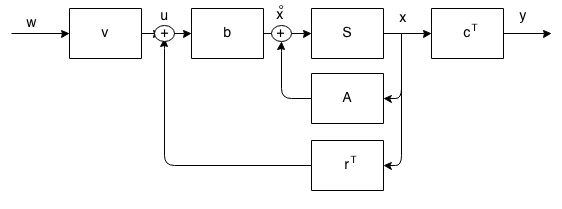
\includegraphics[scale = 0.4]{images/zustandsregler.png}
\end{center}
\subsection{Polvorgabe}
Bei der Polvorgabe werden die Pole des geschlossen Systems vorgegeben.
\[
	A_{CL}=F= A-b\cdot r^T
\]
\[
	A_{CL,R}= A_R-b_R\cdot {r^T}_R	\\	{r^T}_R=
		\begin{bmatrix}
				r_{1,R}	&	r_{2,R}	& \ldots &r_{n,R}\\
		\end{bmatrix}
\]
Daraus folgt:
\[
		A_{CL,R}=
		\begin{bmatrix}
			0 &	1 & 0 & \ldots & 0\\
			0 & 0 & 1 & \ldots & 0\\
			\vdots & \vdots & \vdots & \ddots & \vdots \\
			0 & 0 & 0 & \ldots & 1\\
			-\frac{a_0}{a_n}-r_{1,R}  &-\frac{a_1}{a_n}-r_{2,R} & -\frac{a_2}{a_n}-r_{3,R} & \ldots &\underbrace{-\frac{a_{n-1}}{a_n}-r_{n,R}}_{\textbf{$-c^{n-1}$}}\\	
		\end{bmatrix}
\]
Diese Matrix kann gerade in das Istpolynom überführt werden.
\\
Istpolynom:
\[
	p_{Cl,r}(s)=s^n+
	\underbrace{(a_{n-1}+r_{n,R})	}_{\textbf{$c^{n-1}$}}
	\cdot s^{n-1}+...+(a_{1}+r_{2,R})a_1\cdot s +(a_0+r_{1,r})
\]
Das Sollpolynom ist durch die Nullstellen vorgegeben:
\[\begin{aligned}
	p(s) &= (s-s_1)(s-s_2)\ldots(s-s_n)\\
	&=s^n+p_{n-1}\cdot s^{n-1}+...+p_1\cdot s +p_0
\end{aligned}\]
Koeffizientenvergleich ergibt nun:
\[\begin{aligned}
	r_{1,R}&=p_0-a_0 \\
	r_{2,R}&=p_1-a_1 \\
	r_{n,R}&=p_{n-1}-a_{n-1}
\end{aligned}\]
Die Reglermatrix ist somit gegeben durch:
\[
	r^T={r^T}_R \cdot T_R
\]
Die Reglermatrix kann auch direkt berechnet werden mit:
\[
	r^T = p_0 \cdot q^T_S + \ldots + p_{n-1}\cdot q^T_S A^{n-1} + q^T_S A^n
\]



\subsection{Vorfilter / Vorverstärker}
Der Vorfilter/Vorverstärker gewährleistet, dass im stationärem Zustand $y$ mit dem gewünschtem, konstantem Vektor $w$ übereinstimmt.
\[\begin{aligned}
	 	&v=[c^T(b\cdot r^T-A)^{-1}\cdot b]^{-1} \\
	 	&v_R=[c^T_R(b_R\cdot r^T_R-A_R)^{-1}\cdot b]^{-1}
\end{aligned}\]
\subsection{Beobachter}
Beobachter ist ein Nachbau des System für den Rechner. Er beinhaltet alle Punkte des realen System. Dafür werden keine Sensoren benötigt. Die Variablen werden geschätzt.\\
\\
Das $h$ muss derart bestimmt werden, dass $eigW(A-h_c^T)<0$ sind.\\
\\
Falls das System in BNF vorliegt, gilt:
\[\begin{aligned}
	A_B &= {T_B}^{-1}\cdot A \cdot T_B	\\	
	{c^T}_B &= c^T\cdot T_B = \begin{bmatrix}
		0 & 0 & \ldots & 1
	\end{bmatrix}	\\	
	b_B &= T_B^{-1}\cdot b
\end{aligned}\]
\[
	A_B= \begin{bmatrix}
		0 &	0 & 0 & \ldots & -\frac{a_0}{a_n}\\
		1 & 0 & 0 & \ldots & -\frac{a_1}{a_n}\\
		0 & 1 & 0 & \ldots & -\frac{a_2}{a_n}\\
		\vdots &  & \ddots &  & \vdots \\
		0 & 0 & \ldots & 1 &-\frac{a_{n-1}}{a_n}\\	
	\end{bmatrix}
\]
Folgende Gleichung wird für die Bestimmung des Istpolynoms benötigt. Da $a_n=1$, kann folgende Vereinfachung gemacht werden:
\[
	\dot{e}_{x,B}=(A_B-h_B\cdot c_B^T)\cdot e_{x,B}=
	\begin{bmatrix}
		0 &	0 & 0 & \ldots & -a_0-h_{B,1}\\
		1 & 0 & 0 & \ldots & -a_1-h_{B,2}\\
		0 & 1 & 0 & \ldots & -a_2-h_{B,3}\\
		\vdots &  & \ddots &  & \vdots \\
		0 & 0 & \ldots & 1 &-a_{n-1}-h_{B,n}\\	
	\end{bmatrix}
\]
Istpolynom:
\[
	u(s)=s^n+(a_{n-1}+h_{B,n})s^{n-1}+...+(a_1+h_{B,2})s+(a_0+h_{B,1})
\]
Sollpolynom:
\[
	p(s)=s^n+p_{n-1}s^{n-1}+...+p_1 s+p_0
\]
Aus diesen beiden Gleichungen kann via Koeffizientenvergleich die Matrix $h_B$ bestimmt werden.
\[
	h_{B,1}=p_0-a_0	\\	h_{B,2}=p1-a1	\\	etc.	
\]
\[
	h_B=p-a \\ h=T_B\cdot h_B \\
\]